% Source: graduate-coursework/Research/How_to_write/00_Contrastive_Synthesis.tex
% Description: \textbf{Activity Theory (Engestr\"{o

\documentclass[border=4pt]{standalone}
\usepackage{newtxtext,newtxmath}
\usepackage{tikz}
\usetikzlibrary{arrows.meta,positioning,shapes.geometric,calc,decorations.pathreplacing}

\definecolor{garnet}{HTML}{73000A}
\definecolor{atlantic}{HTML}{466A9F}
\definecolor{congaree}{HTML}{1F414D}
\definecolor{horseshoe}{HTML}{65780B}
\definecolor{rose}{HTML}{CC2E40}
\definecolor{honeycomb}{HTML}{A49137}
\definecolor{warmgrey}{HTML}{676156}
\definecolor{black90}{HTML}{363636}
\definecolor{black70}{HTML}{5C5C5C}
\definecolor{black50}{HTML}{A2A2A2}
\definecolor{black30}{HTML}{C7C7C7}
\definecolor{black10}{HTML}{ECECEC}
\definecolor{sandstorm}{HTML}{FFF2E3}

\begin{document}
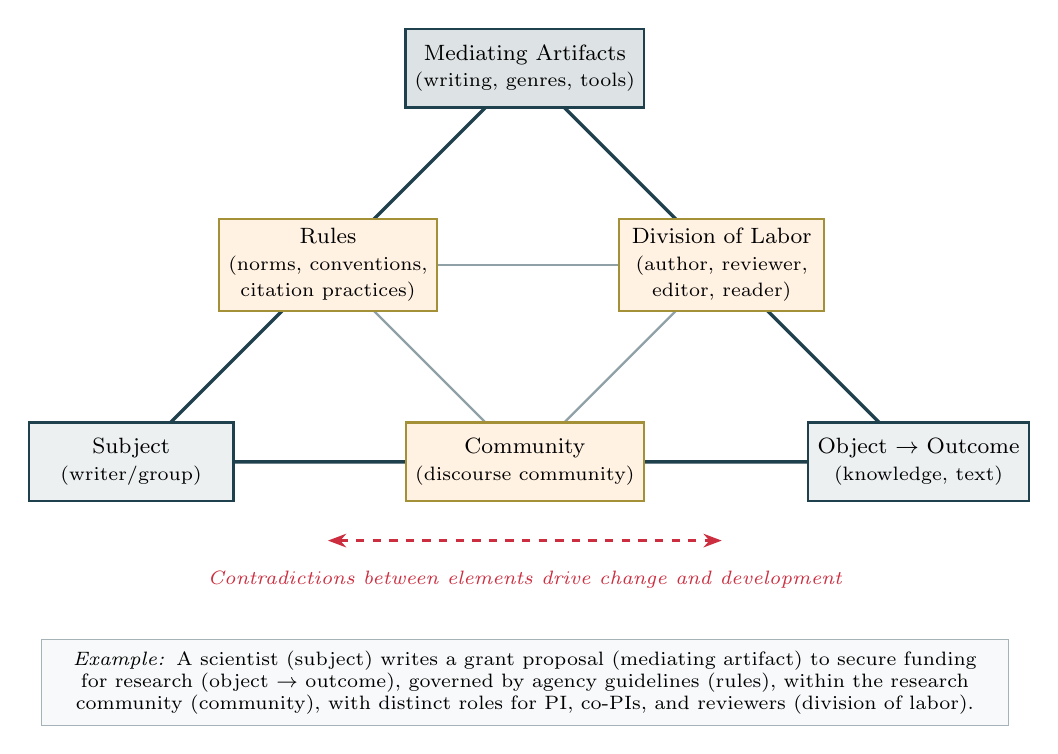
\begin{tikzpicture}[
    every node/.style={font=\footnotesize},
    element/.style={rectangle, draw=congaree, thick, fill=congaree!8,
        minimum width=2.6cm, minimum height=1cm, align=center, font=\footnotesize},
]

% Triangle vertices
\coordinate (top) at (0, 5);
\coordinate (left) at (-5, 0);
\coordinate (right) at (5, 0);

% Triangle edges
\draw[very thick, congaree] (top) -- (left) -- (right) -- cycle;

% Midpoints for lower triangle
\coordinate (midleft) at (-2.5, 2.5);
\coordinate (midright) at (2.5, 2.5);
\coordinate (midbottom) at (0, 0);

% Lower triangle lines
\draw[thick, congaree!50] (midleft) -- (midright);
\draw[thick, congaree!50] (midleft) -- (midbottom);
\draw[thick, congaree!50] (midright) -- (midbottom);

% Nodes at vertices
\node[element, fill=congaree!15] at (top) {Mediating Artifacts\\{\scriptsize (writing, genres, tools)}};
\node[element] at (left) {Subject\\{\scriptsize (writer/group)}};
\node[element] at (right) {Object $\rightarrow$ Outcome\\{\scriptsize (knowledge, text)}};

% Nodes at midpoints
\node[element, fill=sandstorm, draw=honeycomb] at (midbottom)
    {Community\\{\scriptsize (discourse community)}};
\node[element, fill=sandstorm, draw=honeycomb] at (midleft)
    {Rules\\{\scriptsize (norms, conventions,}\\{\scriptsize citation practices)}};
\node[element, fill=sandstorm, draw=honeycomb] at (midright)
    {Division of Labor\\{\scriptsize (author, reviewer,}\\{\scriptsize editor, reader)}};

% Contradictions annotation
\node[font=\scriptsize\itshape, text=rose, align=center] at (0, -1.5)
    {Contradictions between elements drive change and development};
\draw[thick, rose, dashed, {Stealth}-{Stealth}] (-2.5, -1) -- (2.5, -1);

% Example annotation
\node[rectangle, draw=congaree!40, fill=congaree!3, inner sep=4pt,
    font=\scriptsize, align=center, text width=12cm] at (0, -2.8)
    {\textit{Example:} A scientist (subject) writes a grant proposal (mediating artifact) to secure funding for research (object $\rightarrow$ outcome), governed by agency guidelines (rules), within the research community (community), with distinct roles for PI, co-PIs, and reviewers (division of labor).};

\end{tikzpicture}
\end{document}
